\section{Stationary stochastic process White Noise}

Let's explore the general scenario wherein a stationary stochastic process is generated as outputs of digital filters:
\begin{figure}[H]
    \centering
    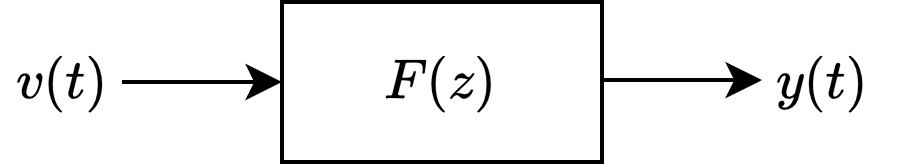
\includegraphics[width=0.45\linewidth]{images/ssp.png}
    \caption{Stationary stochastic process}
\end{figure}
In this setup, $v(t)$ represents a stationary stochastic process, and $F(z)$ is asymptotically stable. 
Consequently, the output $y(t)$ manifests as a stationary stochastic process.
\begin{theorem}
    The spectral density of the output is given by:
    \[\Gamma_y(\omega)=\left\lvert F(e^{j\omega})\right\rvert^2 \Gamma_v(\omega) \]
\end{theorem}

\begin{example}
    Let's examine an MA ($1$) process:
    \[y(t)=e(t)+ce(t-1)\qquad c\in\mathbb{R},e(t)\sim WN(0,1)\]
    The computation of the covariance function is straightforward:
    \[\gamma_y(\tau)=\begin{cases}
        1+c^2 \qquad \tau=0 \\
        c \qquad\qquad\: \tau=\pm 1 \\
        0 \qquad\qquad \left\lvert \tau\right\rvert \geq 1
    \end{cases}\]

    We can compute the spectral density using the definition:
    \begin{align*}
        \Gamma_y(\omega)    &=\sum_{\tau=-\infty}^{+\infty}\gamma_y(\omega)e^{-j\omega\tau} \\
                            &=\gamma_y(0)e^{-j\omega 0} + \gamma_y(1)e^{-j\omega 1} +\gamma_y(-1)e^{-j\omega(-1)} \\
                            &=\gamma_y(0) + \gamma_y(1)e^{-j\omega} +\gamma_y(-1)e^{j\omega} \\
                            &=1+c^2 + ce^{-j\omega} +ce^{j\omega}                  
    \end{align*}
    Utilizing Euler's formula:
    \[\begin{cases}
        e^{-j\omega}= \cos\omega-j\sin\omega \\
        e^{j\omega}= \cos\omega+j\sin\omega
    \end{cases}\]
    We find:
    \begin{align*}
        \Gamma_y(\omega)    &=1+c^2 + ce^{-j\omega} +ce^{j\omega} \\        
                            &=1+c^2 + c\left(\cos\omega-j\sin\omega+\cos\omega+j\sin\omega\right) \\    
                            &=1+c^2 + 2c\cos\omega                               
    \end{align*}

    Alternatively, the spectral density can be computed using the theorem:
    \[\Gamma_y(\omega)=\left\lvert F(e^{j\omega})\right\rvert^2 \Gamma_v(\omega)\]
    In this case, considering $y(t)=e(t)+ce(t-1)=\left(1+cz^{-1}\right)e(t)=F(z)e(t)$ where $F(z)=\left(1+cz^{-1}\right)$, and since the input process $e(t)$ is a White Noise, the spectral density is $\lambda^2=1$.
    \[\Gamma_y(\omega)=\left\lvert F(e^{j\omega})\right\rvert^2 \Gamma_e(\omega)=\left\lvert 1+ce^{-j\omega}\right\rvert^2 \cdot 1\]
    
    Computing the square of a complex number by multiplying it by its conjugate:
    \begin{align*}
        \Gamma_y(\omega)    &=\left\lvert 1+ce^{-j\omega}\right\rvert^2 \\
                            &=\left(1+ce^{-j\omega}\right)\left(1+ce^{+j\omega}\right) \\
                            &=1+c^2+ce^{-j\omega}+ce^{+j\omega} \\
                            &=1+c^2 + 2c\cos\omega
    \end{align*}

    Now, we aim to compute the covariance function using the found spectral density:
    \begin{align*}
        \gamma_y(0)     &=\dfrac{1}{2\pi}\int_{-\pi}^{\pi}\Gamma_y(\omega)e^{j\omega 0}\,d\omega \\
                        &=\dfrac{1}{2\pi}\int_{-\pi}^{\pi}1+c^2 + 2c\cos\omega\,d\omega \\
                        &=\dfrac{1}{2\pi}\left[\int_{-\pi}^{\pi}1\,d\omega+\int_{-\pi}^{\pi}c^2\,d\omega + \int_{-\pi}^{\pi}2c\cos\omega\,d\omega\right] \\
                        &=\dfrac{1}{2\pi}\left[1+c^2 + 2c\int_{-\pi}^{\pi}\cos\omega\,d\omega\right] \\                     
                        &=\dfrac{1}{2\pi}\left[{\left[\left(1+c^2\right)\omega\right]}_{-\pi}^{\pi} + 2c{\left[\sin\omega\right]}_{-\pi}^{\pi}\right] \\ 
                        &=\dfrac{1}{2\pi}\left[2\pi\left(1+c^2\right)\right] \\       
                        &=1+c^2              
    \end{align*}    
\end{example}